\documentclass[letterpaper,12pt]{article}

\usepackage{tabularx} % extra features for tabular environment
\usepackage{amsmath}  % improve math presentation
\usepackage{amssymb}
\usepackage{multirow}
\usepackage{xcolor}
\usepackage{gensymb}
\usepackage{appendix}
\usepackage{verbatim}
\usepackage{bigints}

\usepackage{mathtools}
\usepackage{gensymb}
\usepackage{float}
\usepackage{listings}
\usepackage[export]{adjustbox}
\usepackage[super]{nth}
\usepackage{graphicx} % takes care of graphic including machinery
\usepackage[margin=1in,letterpaper]{geometry} % decreases margins
\usepackage{cite} % takes care of citations
\usepackage[final]{hyperref} % adds hyper links inside the generated pdf file

\newcommand*{\tran}{^{\mkern-1.5mu\mathsf{T}}}
\DeclarePairedDelimiter\ceil{\lceil}{\rceil}
\DeclarePairedDelimiter\floor{\lfloor}{\rfloor}
\hypersetup{
    colorlinks=false,       % false: boxed links; true: colored links
    linkcolor=blue,        % color of internal links
    citecolor=blue,        % color of links to bibliography
    filecolor=magenta,     % color of file links
    urlcolor=blue         
}
%++++++++++++++++++++++++++++++++++++++++++++++++++++++++++++++++++++++++++++++++



%++++++++++++++++++++++++++++++++++++++++++++++++++++++++++++++++++++++++++++++++
% Start modifying the labwork number, your team number and the name and METU id
% of your group members.
\newcommand{\reporttitle}{Solution Set 8}
\newcommand{\reportauthor}{ Volkan Aydıngül (Id: 0075359 )\\
                            }
                            % If any teammate does not help to write this report,
                            % you may not write his/her name here.
%++++++++++++++++++++++++++++++++++++++++++++++++++++++++++++++++++++++++++++++++



%++++++++++++++++++++++++++++++++++++++++++++++++++++++++++++++++++++++++++++++++
% DO NOT MODIFY THIS SECTION
\begin{document}
\begin{titlepage}
\newcommand{\HRule}{\rule{0.7\linewidth}{0.5mm}}
\begin{center} % Center remainder of the page
%	LOGO SECTION

\includegraphics[width = 8cm]{figures/koc_logo.png}

%	HEADING SECTIONS
\textsc{\Large PHYS 514 - Computational Physics}\\[1.5cm] 
%	TITLE SECTION
\HRule \\[0.6cm]
{ \huge \bfseries \reporttitle}\\ % Title of your document
\HRule \\[1.5cm]
\end{center}
\vspace{2cm}
%	AUTHOR SECTION
\begin{flushleft} \large
\textit{Author:}\\
\reportauthor% Your name
\end{flushleft}
\vspace{2cm}
\makeatletter
Date: \@date 
\vfill % Fill the rest of the page with whitespace
\makeatother
\end{titlepage}
%++++++++++++++++++++++++++++++++++++++++++++++++++++++++++++++++++++++++++++++++




\tableofcontents
\newpage





%\begin{figure}[H] 
%   \centering \includegraphics[width=\columnwidth]{figures/figure.png}           
%                \caption{Caption}                
%                   \label{fig:label}
%   \end{figure}


\section{Problem XXIV}
\subsection{Construction of Symmetric Matrix for Neumann Boundary Condition}

\paragraph{} In the \textit{Poisson equation}, the following discretisized form is present:

\begin{equation*}
    u_{j+1,l} + u_{j-1,l} + u_{j,l + 1} + u_{j,l - 1} -4u_{j,l} = h^2\rho_{j,l} 
\end{equation*}
where $u_{j,l}$ and $\rho_{j,l}$ represents the grid points and the forcing terms on a uniform rectangular grid, and $j = 0, \dots, N $ and $l = 0, \dots, M$.

\paragraph{} In the problem construction, the following information is given:
\begin{itemize}
    \item The effective boundary condition is \textit{Neumann boundary condition}.
    \item Discretization scheme is such that $x_i = a + \left(i + \frac{1}{2}\right)\frac{b-a}{N}$ for $i = 0, 1, \dots, N-1$
\end{itemize}

\paragraph{} The first thing that should be done is to observe the behavior of the edges. Because, the intermediate points have always the same structure. For example, the following relation can be observed for edges:

\begin{equation}
    \label{eq:y0dd1}
    u_{j+1,0} + u_{j-1,0} + u_{j,1} + u_{j,- 1} -4u_{j,0} = h^2\rho_{j,0} 
\end{equation}

\begin{equation}
    \label{eq:y0dd2}
    u_{j+1,M-1} + u_{j-1,M-1} + u_{j,M} + u_{j,M - 2} -4u_{j,M-1} = h^2\rho_{j,M-1} 
\end{equation}

\begin{equation}
    \label{eq:yNdd1}
    u_{1,l} + u_{-1,l} + u_{0,l + 1} + u_{0,l - 1} -4u_{0,l} = h^2\rho_{0,l} 
\end{equation}

\begin{equation}
    \label{eq:yNdd2}
    u_{N,l} + u_{N-2,l} + u_{N-1,l + 1} + u_{N-1,l - 1} -4u_{N-1,l} = h^2\rho_{N-1,l} 
\end{equation}


The fact that the $ u_{j,- 1}$, $u_{j,M}$, $u_{-1,l}$, and $u_{N,l}$  are unknown can be immediately observed. To be able to have an idea about the $ u_{j,- 1}$, $u_{j,M}$, $u_{-1,l}$, and $u_{N,l}$, one can easily incorporate the information of the boundary conditions. To be able to simplify the derivation process, the transformation to the one dimensional \textit{dummy variable}, $y$, might be more feasible.

\begin{equation*}
    y'_{-\frac{1}{2}} = \frac{y_{-\frac{1}{2}} - y_{-1}}{\frac{h}{2}} = 0
\end{equation*}

\begin{equation*}
    y'_{-\frac{1}{2}} = \frac{y_{-\frac{1}{2}} - y_{0}}{\frac{h}{2}} = 0
\end{equation*}

\begin{equation*}
    y_{-\frac{1}{2}} = y_{-1}
\end{equation*}

\begin{equation*}
    y_{-\frac{1}{2}} = y_{0}
\end{equation*}

\begin{equation*}
    \boxed{y_{-1} = y_{0}}
\end{equation*}

\paragraph{} Similarly for the end point, the following relation can be hold:

\begin{equation*}
    y'_{N-\frac{1}{2}} = \frac{y_{N-\frac{1}{2}} - y_{N-1}}{\frac{h}{2}} = 0
\end{equation*}

\begin{equation*}
    y'_{N-\frac{1}{2}} = \frac{y_{N-\frac{1}{2}} - y_{N}}{\frac{h}{2}} = 0
\end{equation*}

\begin{equation*}
    y_{N-\frac{1}{2}} = y_{N-1}
\end{equation*}

\begin{equation*}
    y_{N-\frac{1}{2}} = y_{N}
\end{equation*}

\begin{equation*}
    \boxed{y_{N-1} = y_{N}}
\end{equation*}


\paragraph{} Now, it is time to turn back to the \eqref{eq:y0dd1}, \eqref{eq:y0dd2}, \eqref{eq:yNdd1}, and \eqref{eq:yNdd2}. That is, \eqref{eq:y0dd1}, \eqref{eq:y0dd2}, \eqref{eq:yNdd1}, and \eqref{eq:yNdd2} can be written in the following form:

\begin{equation*}
    u_{j+1,0} + u_{j-1,0} + u_{j,1} + u_{j,0} -4u_{j,0} = h^2\rho_{j,0} = u_{j+1,0} + u_{j-1,0} + u_{j,1} -3u_{j,0}
\end{equation*}

\begin{equation*}
    u_{j+1,M-1} + u_{j-1,M-1} + u_{j,M-1} + u_{j,M - 2} -4u_{j,M-1} = h^2\rho_{j,M-1} = u_{j+1,M-1} + u_{j-1,M-1} + u_{j,M - 2} -3u_{j,M-1} 
\end{equation*}

\begin{equation*}
    u_{1,l} + u_{0,l} + u_{0,l + 1} + u_{0,l - 1} -4u_{0,l} = h^2\rho_{0,l} = u_{1,l} + u_{0,l + 1} + u_{0,l - 1} -3u_{0,l} 
\end{equation*}

\begin{equation*}
    u_{N-1,l} + u_{N-2,l} + u_{N-1,l + 1} + u_{N-1,l - 1} -4u_{N-1,l} = h^2\rho_{N-1,l} = u_{N-2,l} + u_{N-1,l + 1} + u_{N-1,l - 1} -3u_{N-1,l}
\end{equation*}

\paragraph{} In this point, one should note that the vertices will be imposed the boundary conditions from the edges, that is, for example:

\begin{equation*}
    u_{1,0} + u_{0,0} + u_{0,1} + u_{0,0} -4u_{j,0} = h^2\rho_{j,0} =  u_{1,0} + u_{0,1} -2u_{j,0}
\end{equation*}

\paragraph{} Moreover, the second derivative for the other data point can be easily expressed as in below form:
\begin{equation*}
    \label{eq:gendd}
    u_{j+1,l} + u_{j-1,l} + u_{j,l + 1} + u_{j,l - 1} -4u_{j,l} = h^2\rho_{j,l} 
\end{equation*}

for $j = 1, \dots, N-2 $ and $l = 1, \dots, M-2$.


\paragraph{} Using all of the aforementioned information here, one can construct the system matrix in lexicographical order as such:

\begin{equation*}
    \begin{bmatrix}
        \mathbf{V} & \mathbf{I} & 0 & 0 & \hdots\\
        \mathbf{I}  & \mathbf{J} & \mathbf{I} & 0 & 0 &\hdots\\
        0  & \mathbf{I} & \mathbf{J} & \mathbf{I} & 0 & 0 &\hdots \\
        0  & 0 & \mathbf{I} & \mathbf{J} & \mathbf{I} & 0 & 0 &\hdots\\
           &   & \ddots  & \ddots   & \ddots  \\ 
           \\
           \\
           \\
        0 & 0 & 0 & 0 &  & \hdots  &   &  \mathbf{I} & \mathbf{J} & \mathbf{I} \\ 
        0 & 0 & 0 & 0 &  & \hdots  &   &  0 & \mathbf{I} & \mathbf{V} \\   
    \end{bmatrix}
\begin{comment}

    \begin{bmatrix}
        y_0 \\
        y_1 \\
        y_2 \\
        \\
        \vdots \\
        \vdots \\
        \\
        y_{N-3} \\
        y_{N-2} \\
        y_{N-1} \\
                
    \end{bmatrix} = 
    \begin{bmatrix}
        \rho_0 \\
        \rho_1 \\
        \rho_2 \\
        \\
        \vdots \\
        \vdots \\
        \\
        \rho_{N-3} \\
        \rho_{N-2} \\
        \rho_{N-1} \\
    \end{bmatrix}
\end{comment}
\end{equation*}

where $\mathbf{V}$ and $\mathbf{J}$ represents:


\begin{equation*}
    \mathbf{V} = \begin{bmatrix}
        -2 & 1 & 0 & 0 & \hdots\\
        1  & -3 & 1 & 0 & 0 &\hdots\\
        0  & 1 & -3 & 1 & 0 & 0 &\hdots \\
        0  & 0 & 1 & -3 & 1 & 0 & 0 &\hdots\\
           &   & \ddots  & \ddots   & \ddots  \\ 
           \\
           \\
           \\
        0 & 0 & 0 & 0 &  & \hdots  &   &  1 & -3 & 1 \\ 
        0 & 0 & 0 & 0 &  & \hdots  &   &  0 & 1 & -2 \\   
    \end{bmatrix}
\begin{comment}
    \begin{bmatrix}
        y_0 \\
        y_1 \\
        y_2 \\
        \\
        \vdots \\
        \vdots \\
        \\
        y_{N-3} \\
        y_{N-2} \\
        y_{N-1} \\
                
    \end{bmatrix} = 
    \begin{bmatrix}
        \rho_0 \\
        \rho_1 \\
        \rho_2 \\
        \\
        \vdots \\
        \vdots \\
        \\
        \rho_{N-3} \\
        \rho_{N-2} \\
        \rho_{N-1} \\
    \end{bmatrix}
\end{comment}
\end{equation*}



\begin{equation*}
    \mathbf{J} = \begin{bmatrix}
        -3 & 1 & 0 & 0 & \hdots\\
        1  & -4 & 1 & 0 & 0 &\hdots\\
        0  & 1 & -4 & 1 & 0 & 0 &\hdots \\
        0  & 0 & 1 & -4 & 1 & 0 & 0 &\hdots\\
           &   & \ddots  & \ddots   & \ddots  \\ 
           \\
           \\
           \\
        0 & 0 & 0 & 0 &  & \hdots  &   &  1 & -4 & 1 \\ 
        0 & 0 & 0 & 0 &  & \hdots  &   &  0 & 1 & -3 \\   
    \end{bmatrix}
\begin{comment}
    \begin{bmatrix}
        y_0 \\
        y_1 \\
        y_2 \\
        \\
        \vdots \\
        \vdots \\
        \\
        y_{N-3} \\
        y_{N-2} \\
        y_{N-1} \\
                
    \end{bmatrix} = 
    \begin{bmatrix}
        \rho_0 \\
        \rho_1 \\
        \rho_2 \\
        \\
        \vdots \\
        \vdots \\
        \\
        \rho_{N-3} \\
        \rho_{N-2} \\
        \rho_{N-1} \\
    \end{bmatrix}
\end{comment}
\end{equation*}

\subsection{Solution of Poisson Equation}

\paragraph{}

\begin{figure}[H]
\centerline{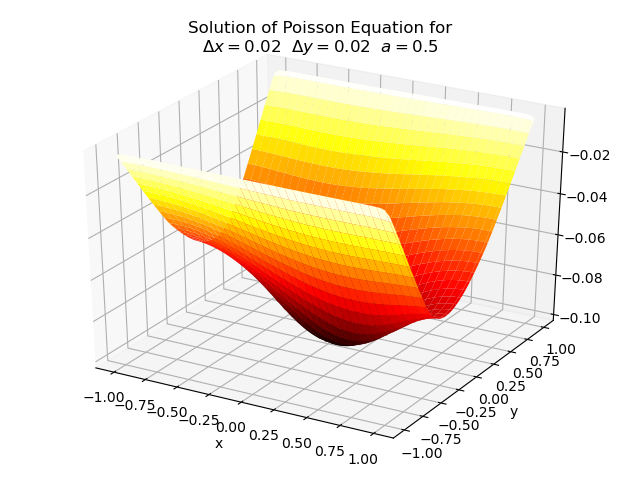
\includegraphics[width=\linewidth]{figures/05.png}}
\caption{Solution of Poisson equation for $a = 0.5$}
\label{fig:05}
\end{figure}
    

\begin{figure}[H]
\centerline{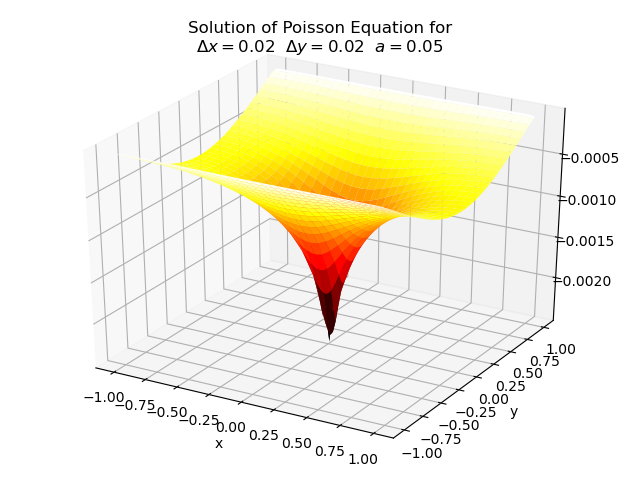
\includegraphics[width=\linewidth]{figures/005.png}}
\caption{Solution of Poisson equation for $a = 0.05$}
\label{fig:005}
\end{figure}

\end{document}



              


